% 
% Annual Cognitive Science Conference
% Sample LaTeX Paper -- Proceedings Format
% 

% Original : Ashwin Ram (ashwin@cc.gatech.edu)       04/01/1994
% Modified : Johanna Moore (jmoore@cs.pitt.edu)      03/17/1995
% Modified : David Noelle (noelle@ucsd.edu)          03/15/1996
% Modified : Pat Langley (langley@cs.stanford.edu)   01/26/1997
% Latex2e corrections by Ramin Charles Nakisa        01/28/1997 
% Modified : Tina Eliassi-Rad (eliassi@cs.wisc.edu)  01/31/1998
% Modified : Trisha Yannuzzi (trisha@ircs.upenn.edu) 12/28/1999 (in process)
% Modified : Mary Ellen Foster (M.E.Foster@ed.ac.uk) 12/11/2000
% Modified : Ken Forbus                              01/23/2004
% Modified : Eli M. Silk (esilk@pitt.edu)            05/24/2005
% Modified : Niels Taatgen (taatgen@cmu.edu)         10/24/2006
% Modified : David Noelle (dnoelle@ucmerced.edu)     11/19/2014
% Modified : Roger Levy (rplevy@mit.edu)     12/31/2018



%% Change "letterpaper" in the following line to "a4paper" if you must.

\documentclass[10pt,letterpaper]{article}

\usepackage{cogsci}
\usepackage{url}

%\cogscifinalcopy % Uncomment this line for the final submission 


\usepackage{pslatex}
\usepackage{apacite}
\usepackage{float} % Roger Levy added this and changed figure/table
                   % placement to [H] for conformity to Word template,
                   % though floating tables and figures to top is
                   % still generally recommended!

%\usepackage[none]{hyphenat} % Sometimes it can be useful to turn off
%hyphenation for purposes such as spell checking of the resulting
%PDF.  Uncomment this block to turn off hyphenation.
\usepackage{graphicx}


%\setlength\titlebox{4.5cm}
% You can expand the titlebox if you need extra space
% to show all the authors. Please do not make the titlebox
% smaller than 4.5cm (the original size).
%%If you do, we reserve the right to require you to change it back in
%%the camera-ready version, which could interfere with the timely
%%appearance of your paper in the Proceedings.

\title{Birds and Words: Exploring environmental influences on folk categorization}
 
\author{{\large \bf Joshua T. Abbott (joshua.abbott@unimelb.edu.au)} \\
 {\large \bf Charles Kemp (ckemp@unimelb.edu.au)} \\
  School of Psychological Sciences,  \\
  University of Melbourne, 3010, Australia}



\begin{document}

\maketitle


\begin{abstract}
How do we name things? What role does frequency of observation and physical size play in categorization of animals? Here we explore these questions using ideas from anthropology and ethnobiology, and utilizing large-scale citizen science datasets.

\textbf{Keywords:} 
ethnobiology; categorization; bird naming
\end{abstract}


\section{Introduction}



Languages around the world include rich systems of names for plants and animals, and each system can be viewed as the outcome of a natural experiment in which generations of speakers have organized their local environment into categories. A classic line of work in cognitive anthropology addresses the question of how named categories reflect the structure of the local environment~\cite{berlin2014ethnobiological}. One prominent theme is that folk taxonomies often align well with Western scientific taxonomies, suggesting that folk taxonomies are shaped more by environmental structure than by the idiosyncratic needs and concerns of a particular culture. 

Much of the cognitively-oriented work on folk biology took place last century, and in recent years new data sets have made it possible to characterize the structure of the environment in ways that were previously difficult or impossible\cite{sullivan2009ebird,wilman2014eltontraits}.
 Here we draw on these resources to revisit the classic question of the relationship between named categories and the environment. We focus on birds in particular, and begin by compiling properties of the bird species in a given area (e.g.\ how big is each species, and how often is it observed?) We then study how these properties relate to named bird categories in the local language. In particular, we ask whether the frequency of a species influences whether the species is named, and if so whether frequency influences the form of the name for that species and how many other species it is grouped with. 

The effects of frequency on categorization have been previously studied in the psychological literature~\cite{parducci83,nosofsky88,barsalouhl98}.  One relevant finding is that categories tend to be relatively broad in low-frequency regions of stimulus space, but relatively narrow in regions including frequently encountered stimuli~\cite{parducci83}. We might therefore predict that bird species encountered frequently are more likely to be assigned to their own distinctive categories.  

Our focus on frequency also connects with a prominent debate between \emph{intellectualist} ~\cite{berlin2014ethnobiological} and \emph{utilitarian} \cite{hunn1982utilitarian} accounts of folk classification. The intellectualist view holds that named categories reflect ``fundamental biological discontinuities'' that are perceptually salient (Berlin, 1992 p 53)~\nocite{berlin2014ethnobiological}, and assigns a minimal role to freqeuncy. The utilitarian view emphasizes ways in which categories are useful for a given culture, and naturally accommodates frequency effects because assigning a label to a category is especially worthwhile if there are many occasions to use it.

The next section introduces the data sets that we use, and we then address two broad questions. First, we focus on category extensions, and ask whether environmental factors predict whether a species is named, and how the set of named species is organized into groups. Second, we focus on category labels, and ask whether environmental factors predict the relative lengths of category labels, and which labels have the structure of unmarked prototypes. 

%The outline for the rest of the paper is as follows. First we describe some of the factors that ethnobiologists have explored and the variables in particular that we will consider. Then we examine some questions using this data. We then discuss the implications of this work and potential future directions. We conclude with a brief summary of the work.


%What role does frequency of exposure have in being able to determine the name for a bird or its role in a taxonomy? What about the size of the bird? BIG QUESTION: What contributes to naming data?

%More generally, we're interested in exploring computational principles that guide the naming and structuring of categories. Following a tradition of ethnobiological classification \cite{berlin1973general,berlin2014ethnobiological}, we aim to explore what kinds of features influence these behaviors. 

% In particular we will explore frequency of observation. (WE'LL WANT SOME COGPSYCH PAPERS ABOUT THIS -- THAT ACTUALLY MIGHT BE A NICE WAY TO FRAME SOME RESULTS LATER -- SHOULD EXPLORE PREVIOUS PAPERS FOR POSSIBLE HYPOTHESES/PREDICTIONS RELATED TO THIS -- e.g., where we use eBird data as the frequency and test predictions against the language data)

%What ebird can contribute to the folk biology literature: frequency data.

%This connects with the theoretical debate about cognitive vs utilitarian view of classification \cite{hunn1982utilitarian,lopez1997tree}. Frequency data provide some new ways to test the utilitarian view. For example, we could use frequencies to address questions like:
%
%1) do unnamed species tend to have low frequency?
%
%2) if a species is lumped in with another species under the same label -- does one of these species have low frequency?
%
%3) in cases where nomenclature reveals prototype effects -- is the prototype highest in frequency?
%
%We also examine the contribution of mass, following \cite{hunn1999size}, and extending to other questions.
%
%We focus on two issues:
%
%(1) which categories get named
%
%(2) which labels are chosen for those categories


%\section{Environmental factors in ethnobiological classification}

\section{Data sets}

%Environmental factors have played a major role in scientific classification of species \cite{amadon1943bird,hunn1999size}.
%Here we talk about the data we use. We show how to utilize publicly available digitized information to explore these questions.

The literature contains detailed folk classifications of birds from several languages around the world, and we focus here on named bird categories from Zapotec \cite{hunn2008zapotec}, a language spoken in Oaxaca, Mexico.  We used two data sets that characterize the frequency and size of bird species found in Oaxaca, and a third that specifies how these species are organized into named categories.

\subsection{Frequency data}

Our frequency data are drawn from eBird, a citizen-science based bird observation network managed by the Cornell Lab of Ornithology \cite{sullivan2009ebird}.  eBird data are contributed by bird lovers (both professional and amateur) who use the site to record the time and place of bird sightings.  We used data from just the region containing the state of Oaxaca, Mexico\footnote{We used all eBird observation of frequency from the Basic Dataset (EBD) on https://ebird.org/data/download, last accessed January 24, 2020.}. An observer who sees a group of 5 vultures may record both the species (e.g.\ \emph{Cathartes aura}) and the number of birds in the group (5), but we treated each case like this as a single observation of the species in question. Our data for Oaxaca include 660,223 unique observations of 922 distinct species. 

We will take eBird counts as a very rough proxy for the frequency with which a species is encountered in the course of regular life. The fact that nocturnal species will tend to have lower counts than equally common diurnal species is therefore a strength of the data rather than a limitation. eBird, however,  does not provide an unbiased measure of frequency in everyday life. As a group, eBird contributors are more interested in some species than others, and counts for rare but iconic species (e.g.\ the Bald eagle in the USA) will overestimate the frequency which which they are encountered relative to other species. Even so, eBird is a valuable resource that allows rough estimates of a variable (frequency) that would otherwise be extremely difficult to measure.  


\subsection{Size data}
% Bird weights as an aid in taxonomy \cite{amadon1943bird}.
Beyond frequency it is plausible that physical and behavioral characteristics of birds both influence folk categorization.  \citeA{hunn1999size} has documented that smaller species are more likely to be lumped together into large categories, and larger species are more likely to be given distinct names. Following his lead we evaluate bird size as an influence on categorization, and use size data from EltonTraits~\cite{wilman2014eltontraits} which includes information on key attributes for all 9993 extant bird species, including those from Oaxaca.  We use the body mass variable, separately sourced from \cite{dunning2007crc}, which is defined as the geometric mean of average values provided for both sexes. Beyond body mass EltonTraits includes variables related to diet types, foraging strata, and activity patterns, and future studies can explore whether and how these variables influence naming. 


\subsection{Naming data}

Our naming data are based on a detailed folk taxonomy provided by \citeA{hunn2008zapotec}\footnote{
Also available online at \url{http://faculty.washington.edu/hunn/zapotec/z5.html}} based on his fieldwork in San Juan Gb\"{e}\"{e}, a small village in Oaxaca.

Describe the dataset and what we extracted from it (e.g., basic-level, terminal-level names, prototypes, etc.) in more detail here.

For example, the folk-generic name for hummingbirds is \textit{dz\v{i}n\b{g}}, which covers 13 birds in Zapotec. Of these 13 birds, there are 3 other labels besides \textit{dz\v{i}n\b{g}}, there are folk-specifics \textit{dz\v{i}n\b{g}-d\'{a}n-y\v{a}-gu\`{i}}, \textit{dz\v{i}n\b{g}-gu\'{e}}, \textit{and dz\v{i}n\b{g}-y\v{a}-gu\`{i}}.


% \subsection{Distribution of data}
% Here we plot the log mass by log frequency of the birds named in Zapotec in Figure \ref{fig-birdmassxfreq}. We see that smaller birds tend to never have a low frequency.

% \begin{figure}[h!]
%   \begin{center}
%     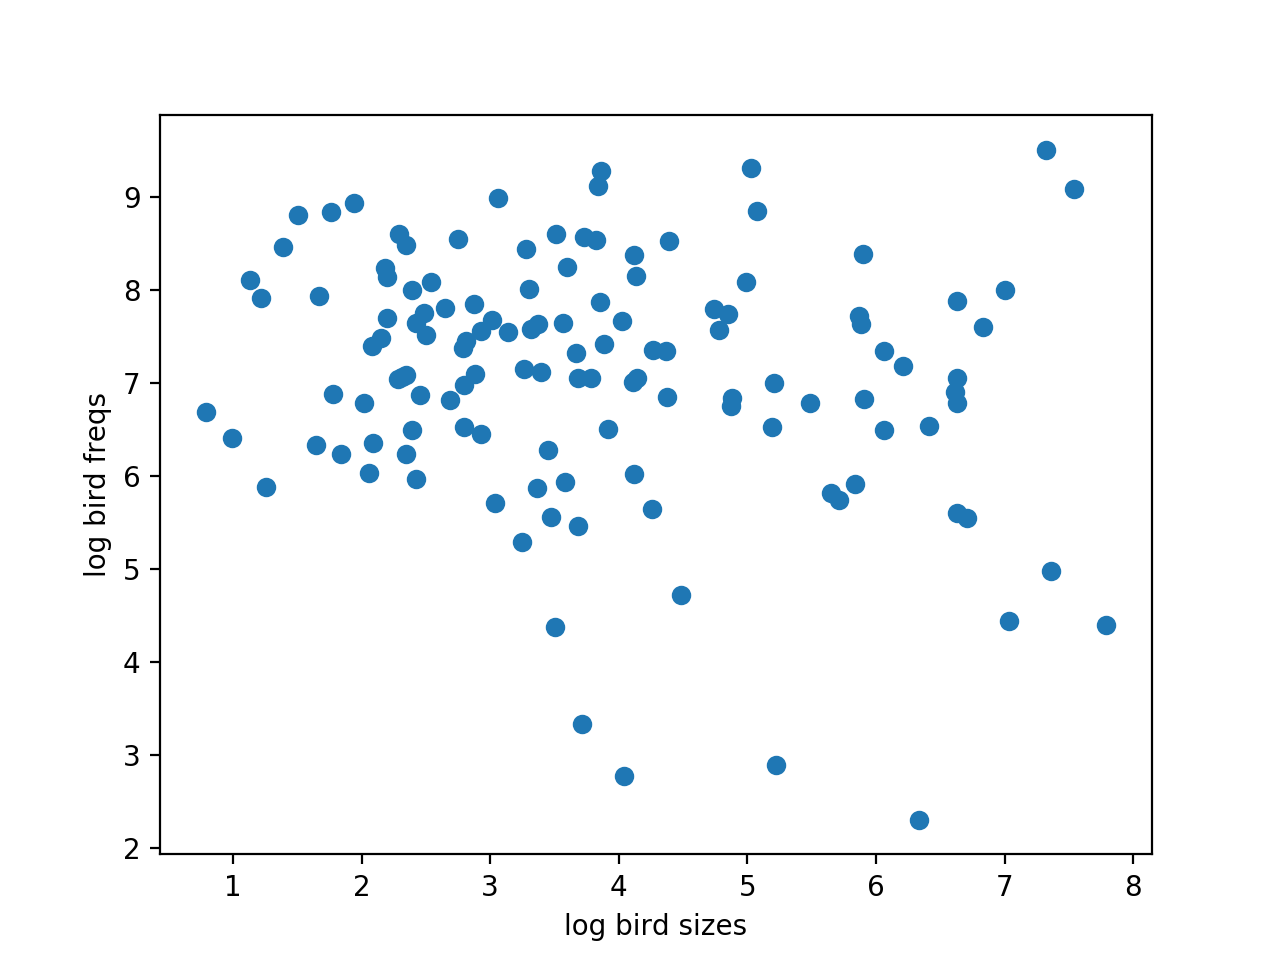
\includegraphics[width=0.5\textwidth]{./figures/bird_massxfreq.png}
%         \caption{Frequencies and masses of birds named in Zapotec.}
%         \label{fig-birdmassxfreq}
%   \end{center}
% \end{figure}


\section{What categories are given a name?}

We first look at the distributions of birds with and without names in Zapotec, using the two environmental factors, in relation to all birds seen in OAX.


\subsection{Frequency}
We first analyze whether the frequency of a species influences if the species is named. We plot the frequency densities of birds named and unamed birds, along with all birds observed in the state of Oaxaca in Figure~\ref{fig-birdfreqviolin}.

\begin{figure}[h!]
  \begin{center}
    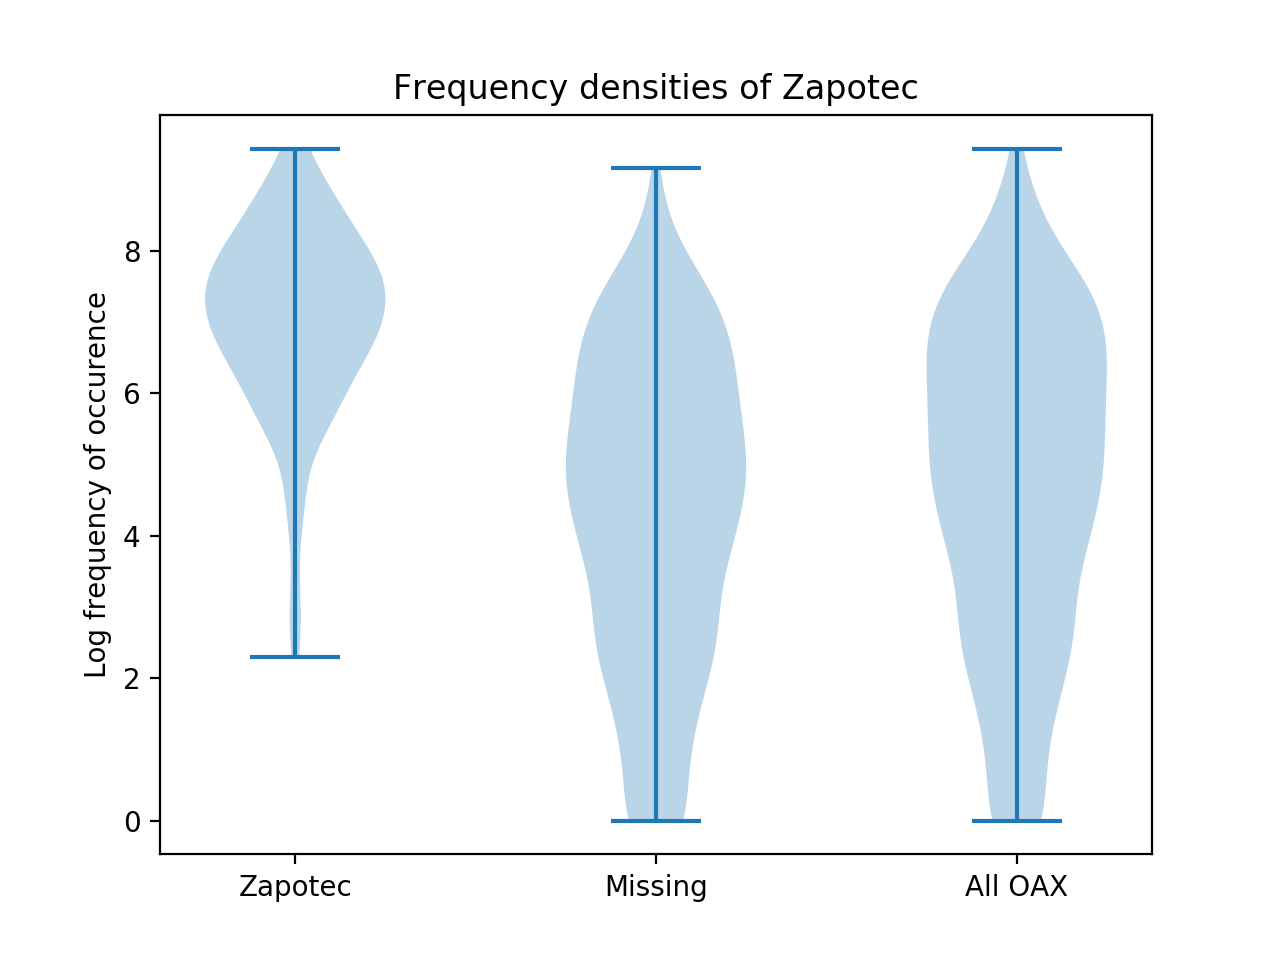
\includegraphics[width=0.5\textwidth]{./figures/birdfreq-violinplots.png}
        \caption{Frequency densities of birds named in Zapotec and those observed in the state of OAX.}
        \label{fig-birdfreqviolin}
  \end{center}
\end{figure}

Here we find that birds named in Zapotec tend to be the most frequently observed birds in Oaxaca. STATS?. This implies XYZ.

\subsection{Size}
Next we analyze the masses of birds named in Zapotec. We plot the densities of birds named and unamed birds, along with all birds observed in the state of Oaxaca in Figure~\ref{fig-birdmassviolin}.

\begin{figure}[h!]
  \begin{center}
    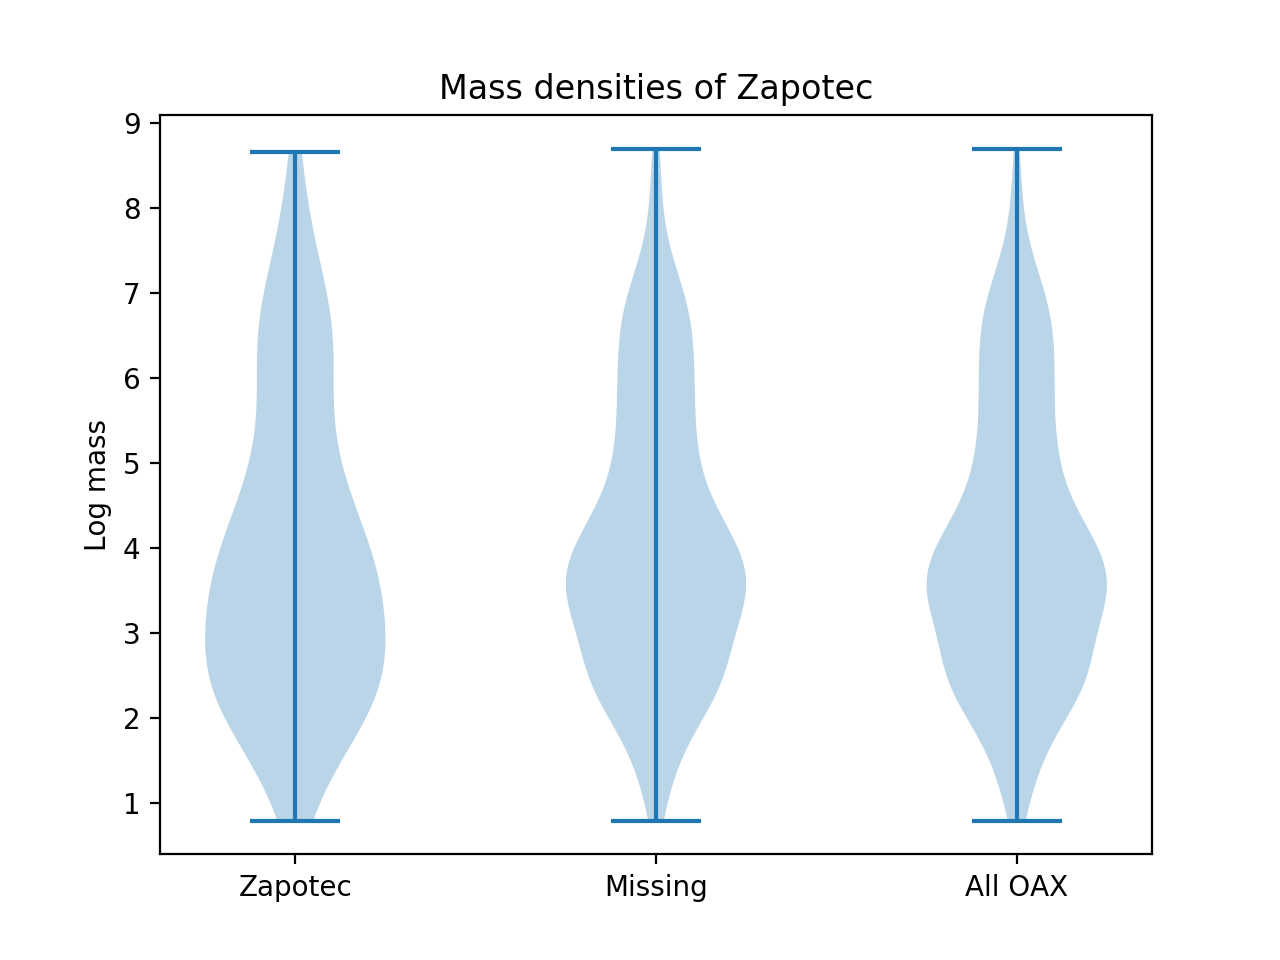
\includegraphics[width=0.5\textwidth]{./figures/birdmass-violinplots.png}
        \caption{Mass densities of birds named in Zapotec and those observed in the state of OAX.}
        \label{fig-birdmassviolin}
  \end{center}
\end{figure}
% \begin{figure*}[hbt!]
%   \begin{center}
%     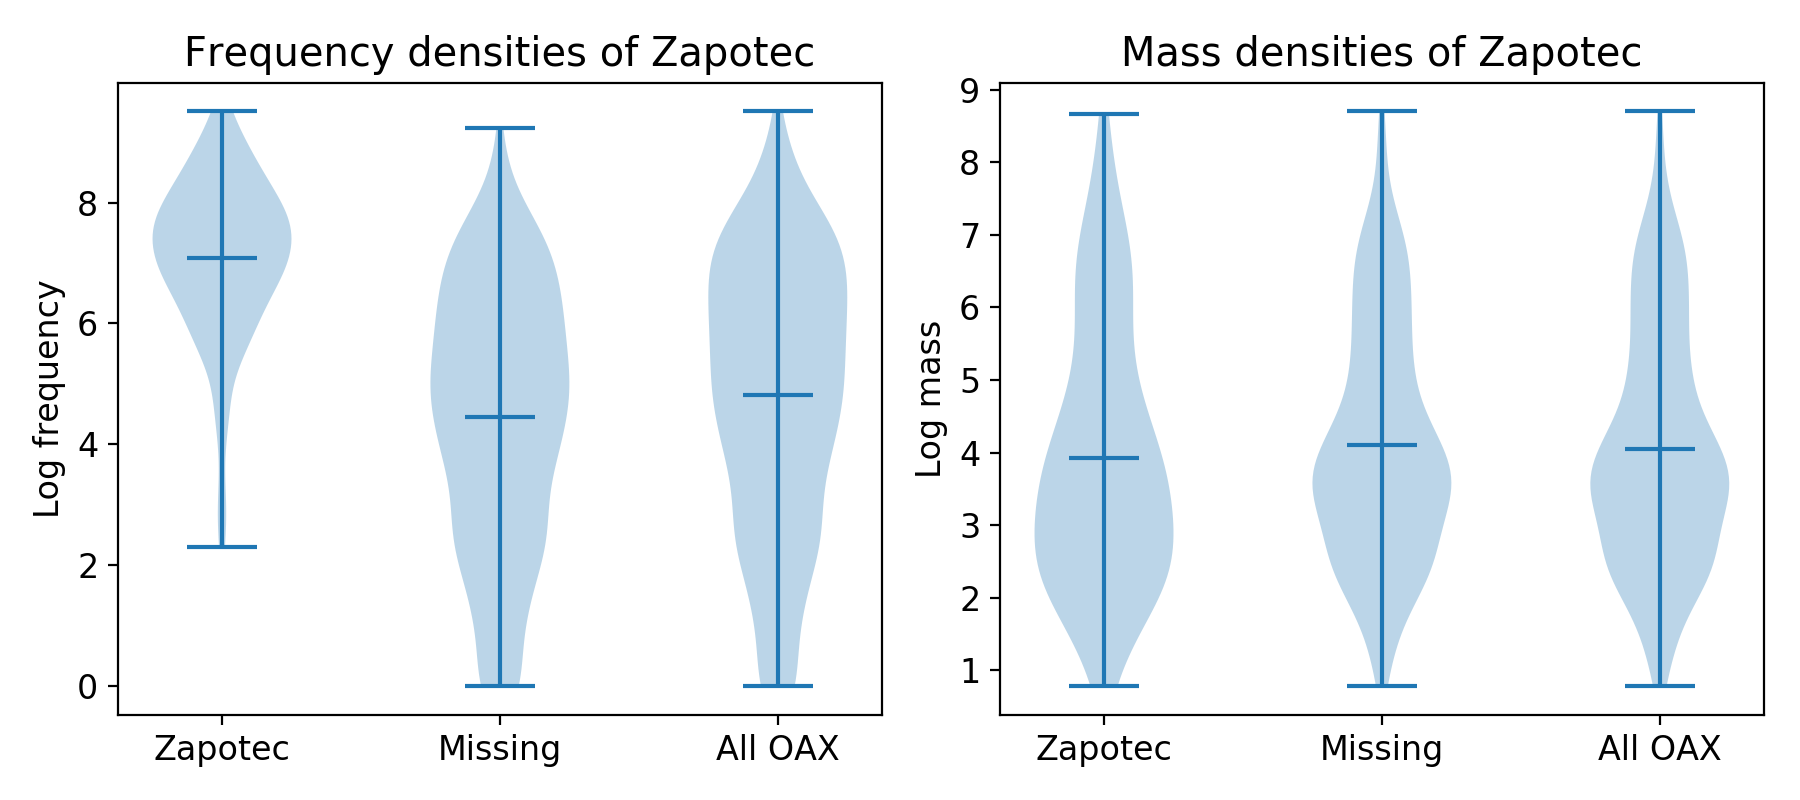
\includegraphics[width=.95\textwidth]{./figures/birdfreqmass-violinplots.png}
%         \caption{Frequency densities (left) and Mass densitities (right) of birds named in Zapotec and those observed in the state of OAX.}
%         \label{fig-birdfreqmassviolin}
%   \end{center}
% \end{figure*}

We see here that frequency is more informative than mass in predicting which birds in Oaxaca are given a name in Zapotec. In the next section, we will find a different set of results.

% mention that information about unnamed species not systematically included in folk taxonomies

\section{Hunn Analysis}
Here we re-explore Hunn's analysis of how size affects the perceptual salience for folk biological classification, following the chapter \cite{hunn1999size}. In sum, he demonstrates a positive correlation between the groupings of named categories, and the average size of those organisms in those categories.

% The Tlingit bird names listed above include several apparent synonyms, terms that differentiate male and female, adult and immature, as well as super- ordinate terms for ‘bird’/‘fowl’ and ‘duck’. 88 named categories of Tlingit birds may be considered ‘basic’ or ‘folk generic’ categories (compare Berlin, 1992), comparable in many respects to the species taxa of academic ornithologists.
% By contrast, ornithologists have recorded 291 species of birds from south- eastern Alaska, the homeland of the Tlingit people (Armstrong, 1990). Have the Tlingit noted only 30 per cent (89/291) of the region’s bird species? By contrast, the Fore of Papua New Guinea name 92 per cent of the species recorded during a comprehensive ornithological survey (Diamond, 1966). These percentages are what Hunn (1975) has defined as the Scientific Species Recognition Ratio (SSRR; Table 13.1), which is the number of bird categories recognized by the local residents divided by the number of bird species recorded in the same territory by professional biologists (Hunn, 1999). This ratio will include a certain number of folk categories that are in 1:1 correspon- dence with a single scientific species, but also instances of under-differentiation – where the folk system ‘lumps’ a group of birds that professional scientists consider to represent two or more species – and over-differentiation – where the folk system ‘splits’ a single scientific species into two or more basic categories. The SSRR will decline when local people are selective in their atten- tion, dismissing species of limited cultural salience with a very general term or ignoring them altogether.
Hunn proposed that the size of an organism is influential in folk categorization and developed a measure which examines the degree to which the organisms are recognized taxonomically in the folk classification. Typical use of the measure considers how many scientific species are included within each folk-generic or folk-specific level taxon. Hunn called this the Scientific Species Recognition Ratio (SSRR).

% For example, the folk-generic name for hummingbirds is \textit{dz\v{i}n\b{g}}, which covers 13 birds in Zapotec. Of these 13 birds, there are 3 other labels besides \textit{dz\v{i}n\b{g}}, there are folk-specifics \textit{dz\v{i}n\b{g}-d\'{a}n-y\v{a}-gu\`{i}}, \textit{dz\v{i}n\b{g}-gu\'{e}}, \textit{and dz\v{i}n\b{g}-y\v{a}-gu\`{i}}. Thus the SSRR of hummingbirds for folk-generic analyses would be 1/13, and 4/13 for folk-specific analyses.

Treating each scientific species as a ``sampling unit'' (the single species point method), calculating an average size for each species, then calculating the SSRRS of each species according to a slightly variant procedure.

The SSRR of a species this procedure is 1 if it corresponds 1:1 to a basic folk taxon, it is 0.5 if it is one of two species included within a single basic folk taxon; it is 0.33 if it is one of three such species; and so on.

We analyze this using both mass and frequency as predictors. Figure~\ref{fig-ssrr} presents SSRR plots of folk-generic names (top row) and folk-specific names (bottom row) for both mass (left column) and frequency (right column).

% \begin{figure*}[t!]
%   \begin{center}
%     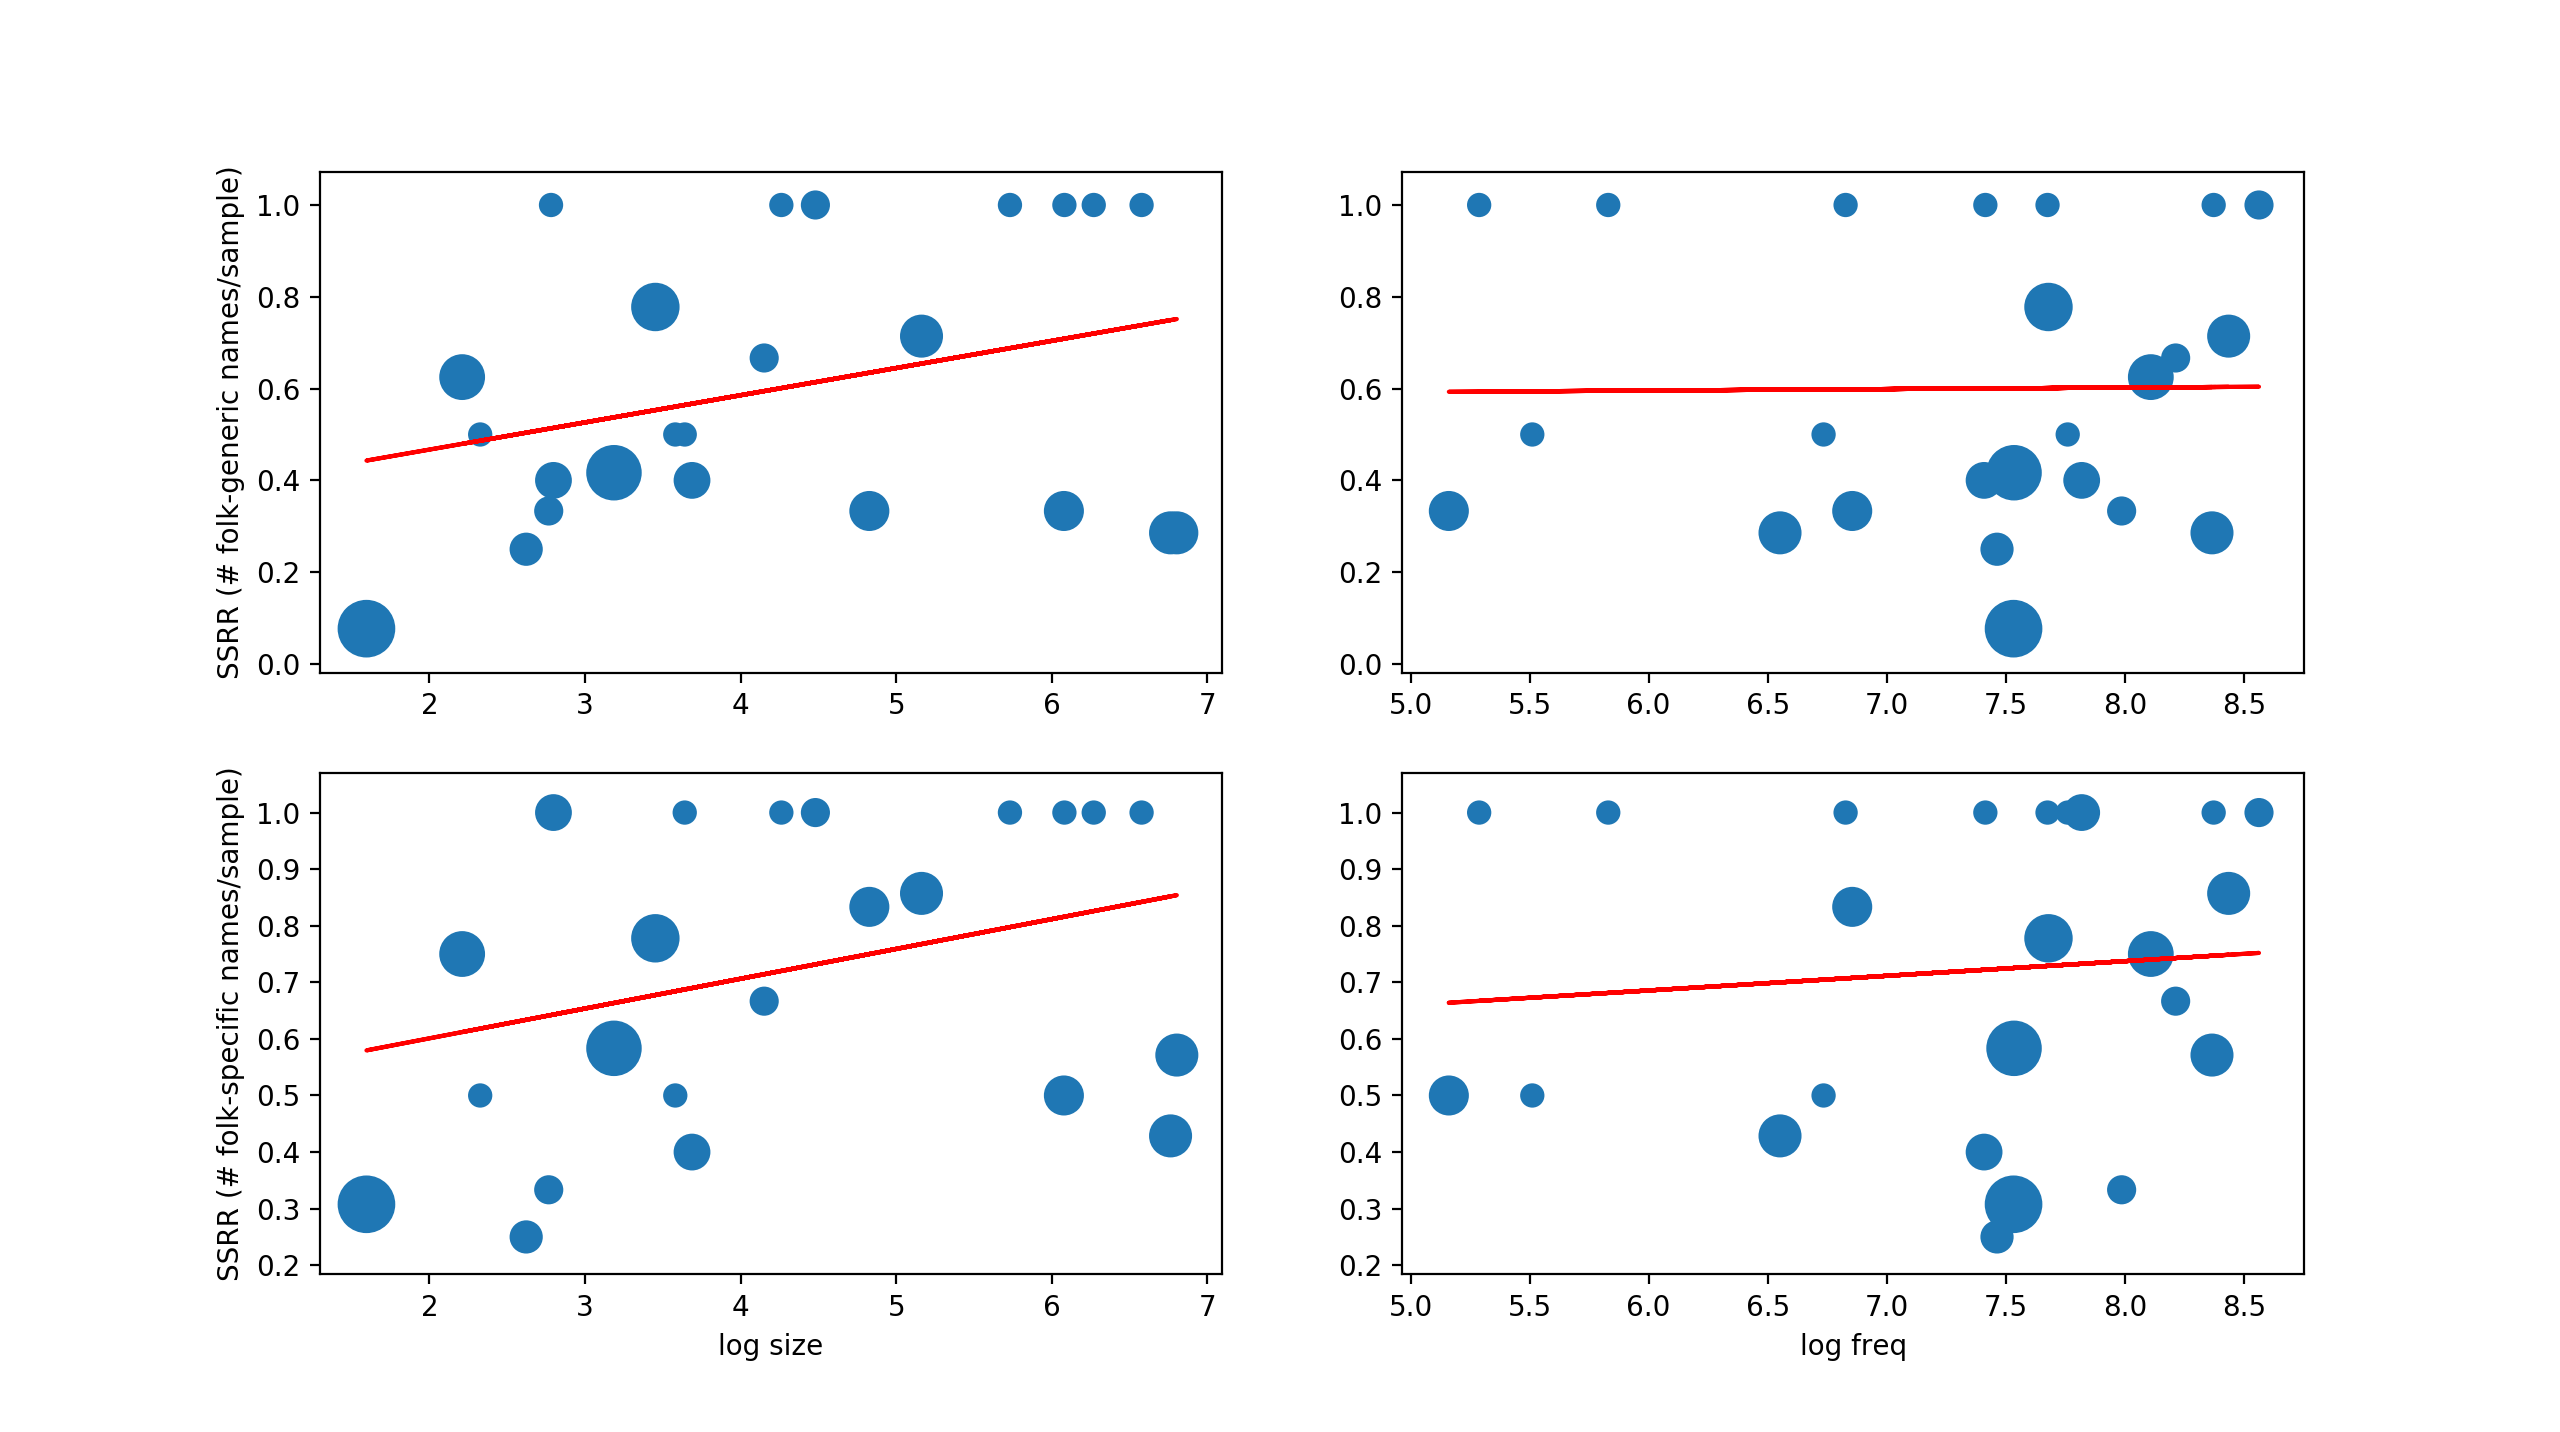
\includegraphics[width=1.0\textwidth]{./figures/ssrr-bothplots.png}
%         \caption{SSRR plots of folk-generic names (top row) and folk-specific names (bottom row) for both mass (left column) and frequency (right column).}
%         \label{fig-ssrr}
%   \end{center}
% \end{figure*}
\begin{figure*}[t!]
  \begin{center}
    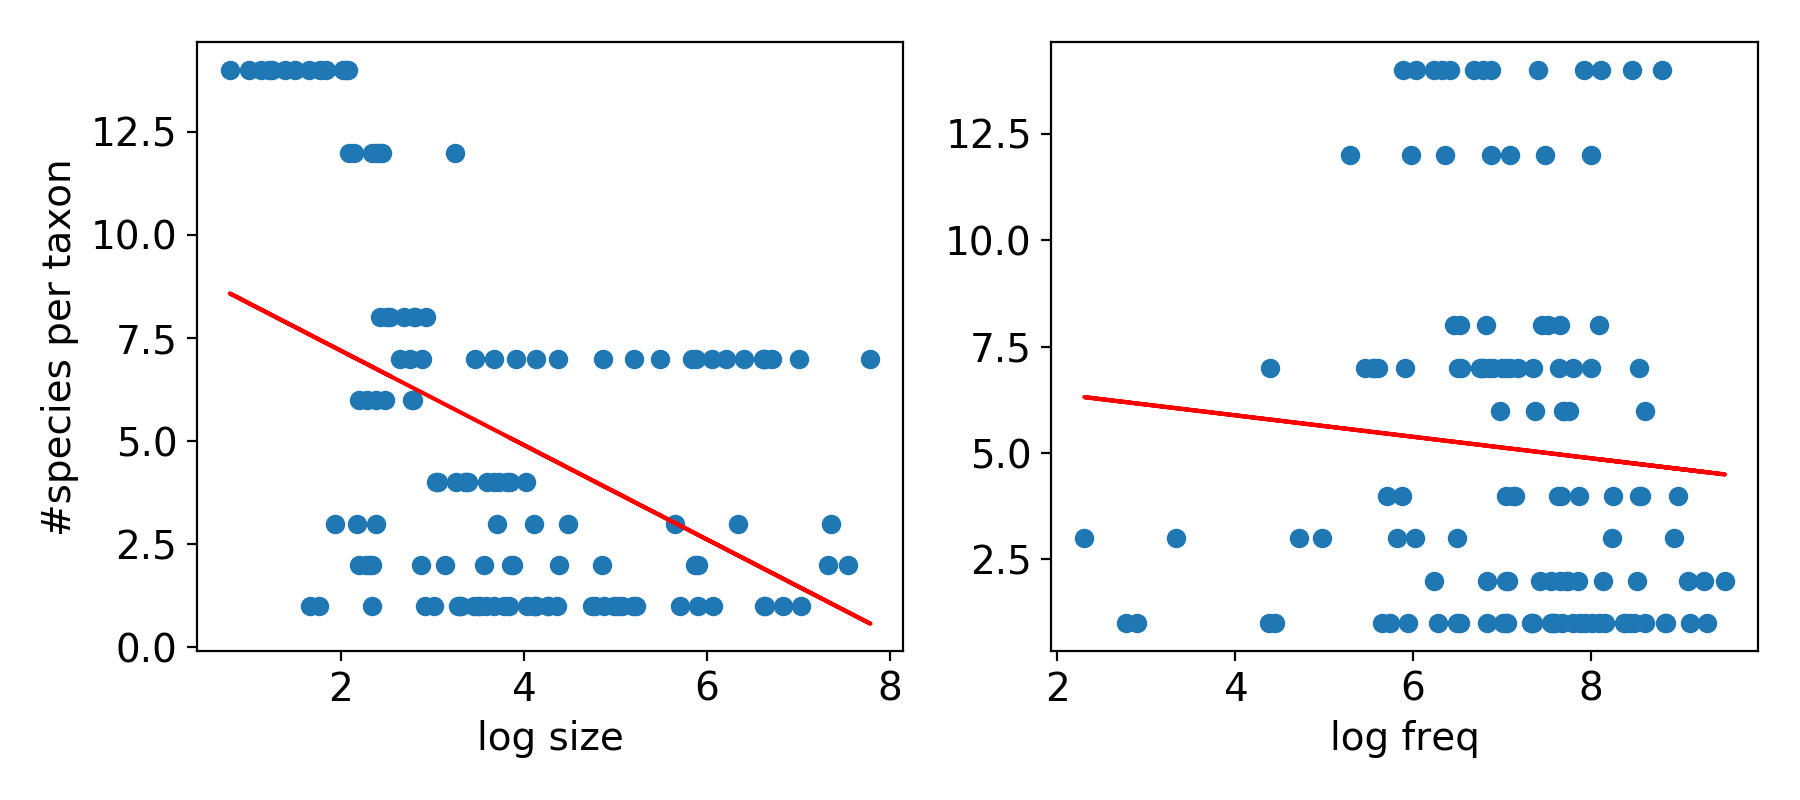
\includegraphics[width=0.95\textwidth]{./figures/ssrr-singlespecies.png}
        \caption{SSRR plots of single-species for both mass (left column) and frequency (right column).}
        \label{fig-ssrr}
  \end{center}
\end{figure*}

Here we find that mass rather than frequency is a better predictor, opposite of the results in the previous section.





\section{Analysis of name-forms}

\subsection{Name-length}
Here we analyze the frequencies of birds named in Zapotec in relation to the name length of the bird. See Figure~\ref{fig-freq-namelength}

\begin{figure}[ht!]
  \begin{center}
    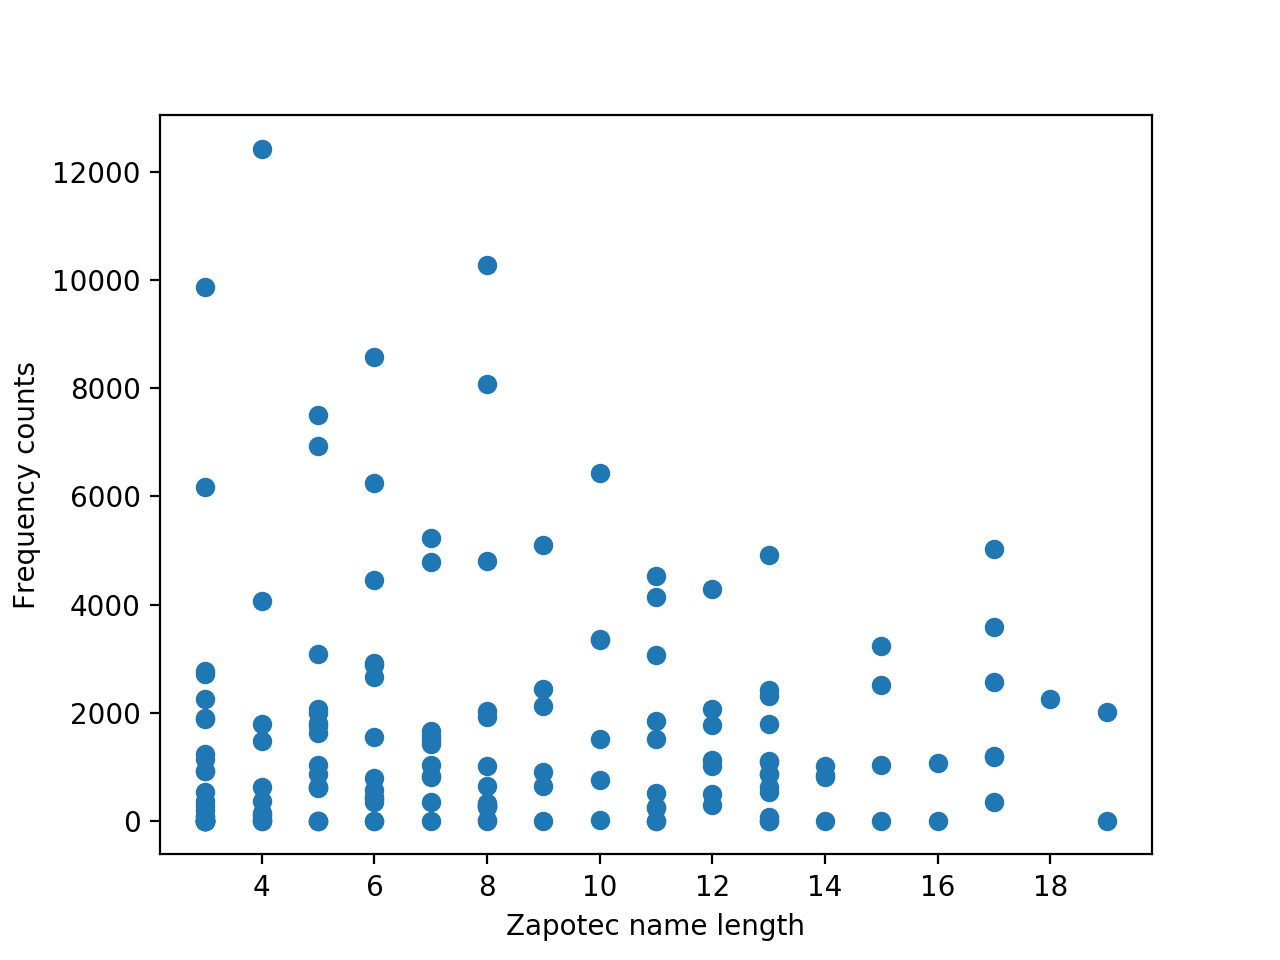
\includegraphics[width=0.5\textwidth]{./figures/freq-namelength.png}
        \caption{Frequency densities of birds named in Zapotec as a function of name length.}
        \label{fig-freq-namelength}
  \end{center}
\end{figure}

\subsection{Compound names}
Here we further examine names based on whether the Zapotec label is a single word (a monomial) or a compound of multiple words. First we examine frequencies, in Figure~\ref{fig-both-nameforms}. Here we see that the monomials tend to be more frequently observed than compounds. The raw mean frequency counts are mono = 2465 and compound = 1715, for monomials and compound names, respectively.

% \begin{figure}[h!]
%   \begin{center}
%     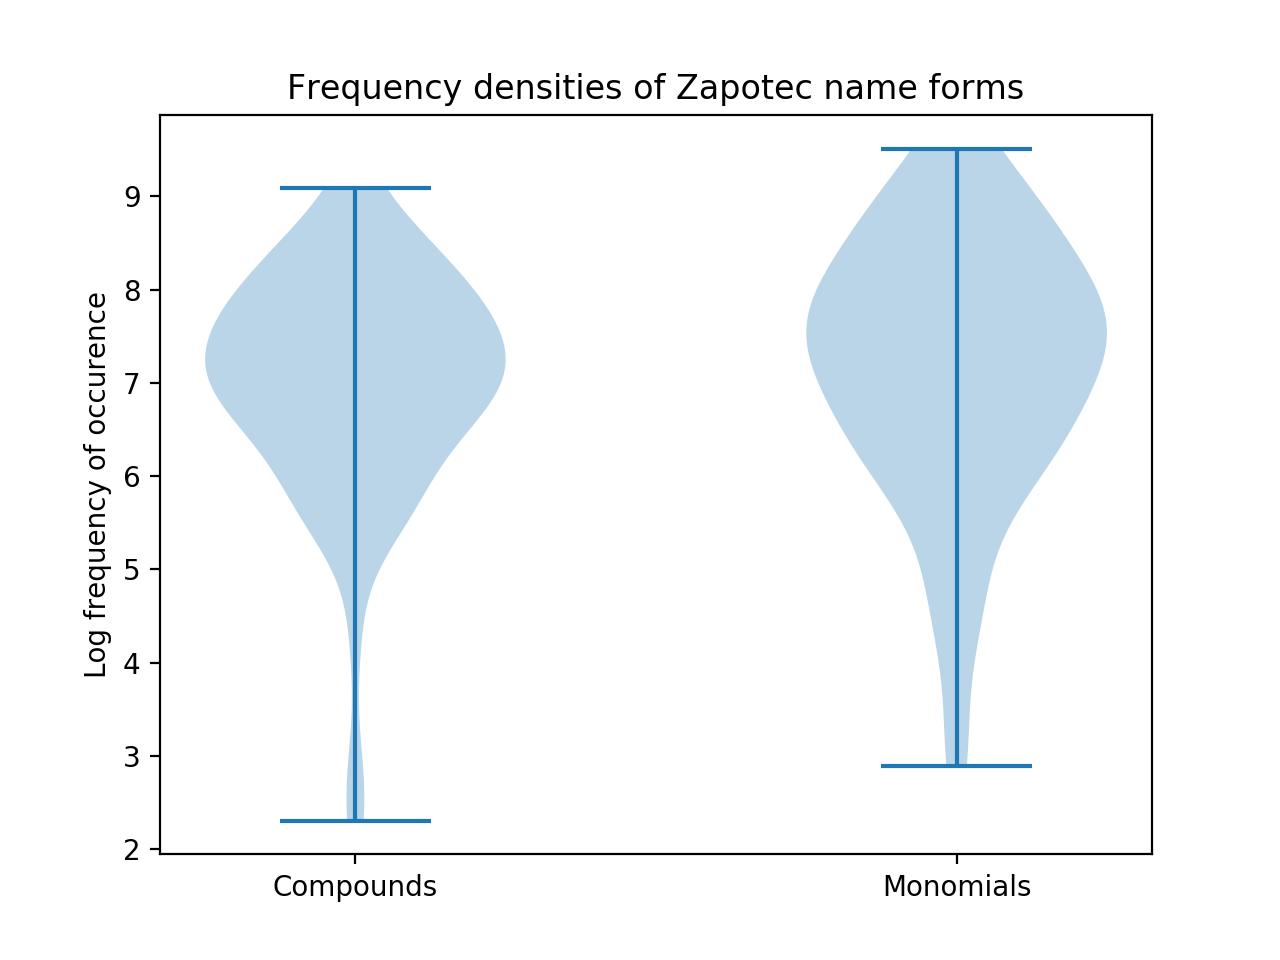
\includegraphics[width=0.5\textwidth]{./figures/freq-nameforms.png}
%         \caption{Frequency densities of birds named in Zapotec as a function of name form.}
%         \label{fig-freq-nameforms}
%   \end{center}
% \end{figure}

We also explore how masses are distributed based on name form. See Figure~\ref{fig-both-nameforms}. Here we see a similar trend as before, with raw mean masses of mono = 375g and compound = 152g.

% \begin{figure}[h!]
%   \begin{center}
%     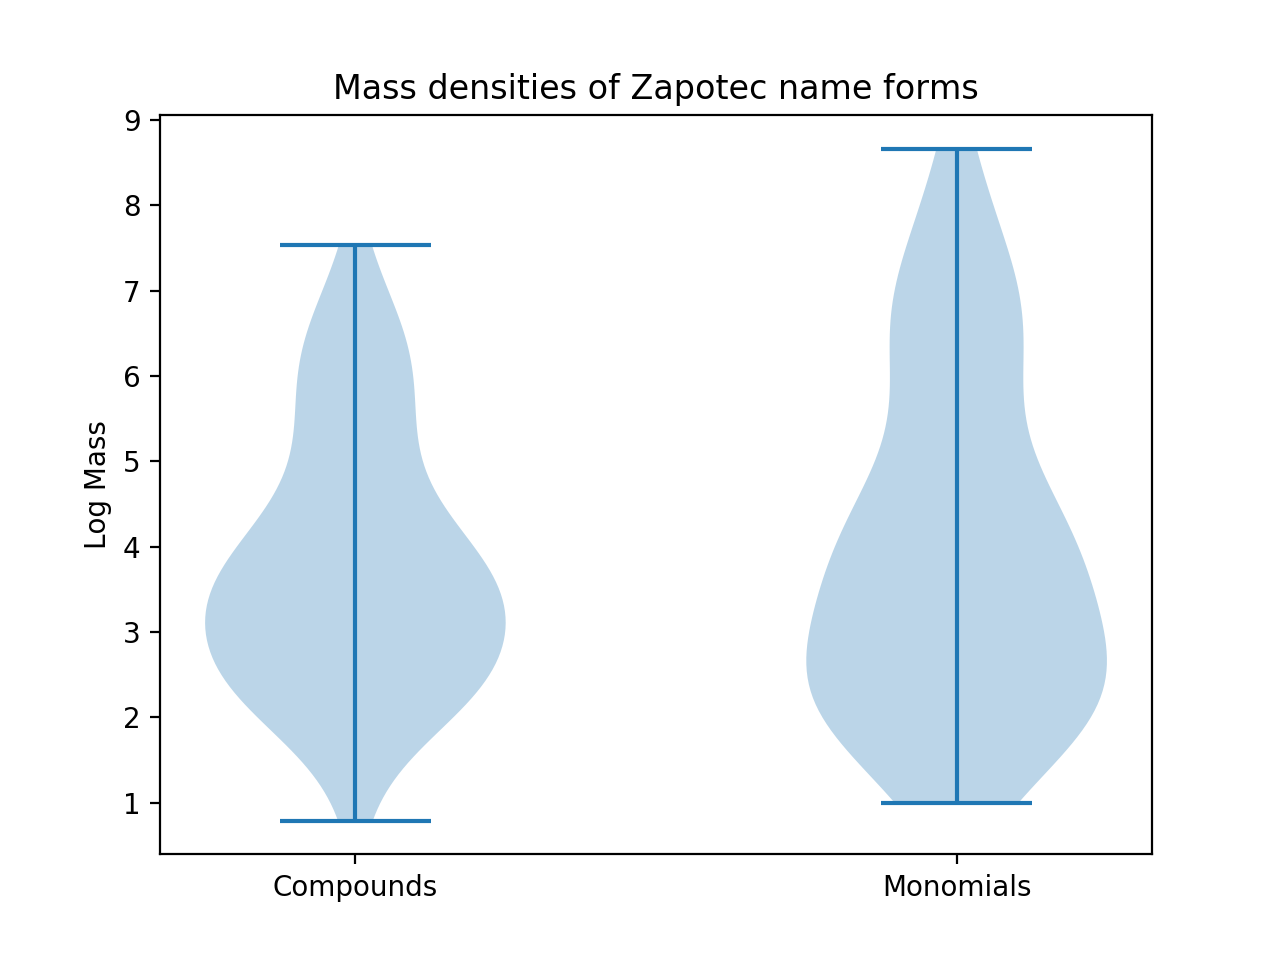
\includegraphics[width=0.5\textwidth]{./figures/mass-nameforms.png}
%         \caption{Mass densities of birds named in Zapotec as a function of name form.}
%         \label{fig-mass-nameforms}
%   \end{center}
% \end{figure}

\begin{figure*}[ht!]
  \begin{center}
    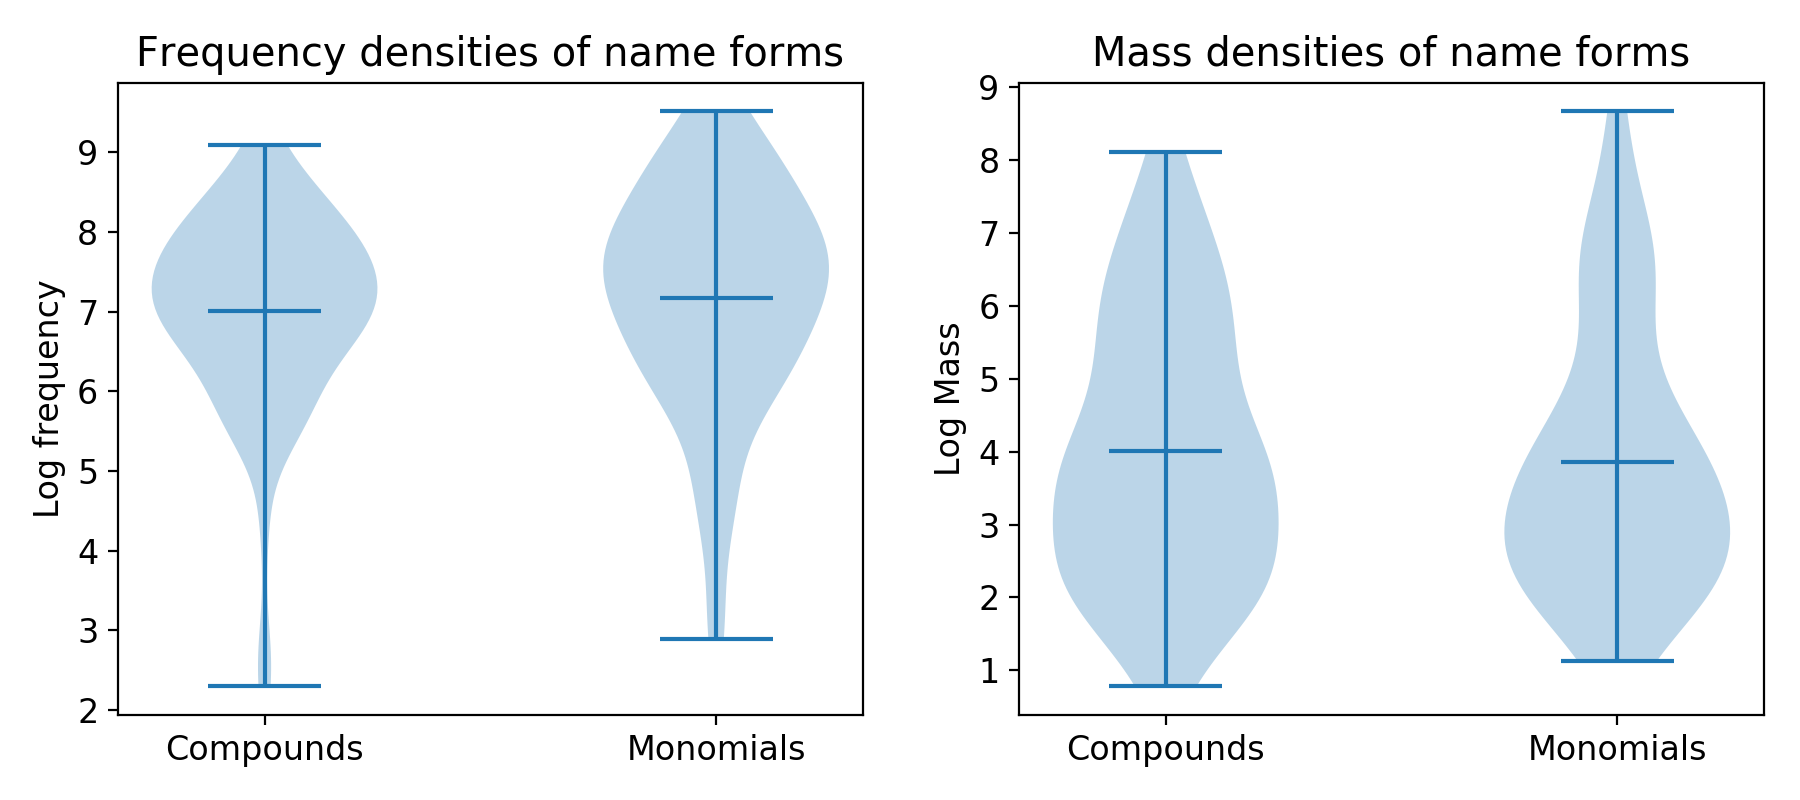
\includegraphics[width=0.95\textwidth]{./figures/nameforms-both.png}
        \caption{Frequency and mass densities of birds named in Zapotec as a function of name form.}
        \label{fig-both-nameforms}
  \end{center}
\end{figure*}

\subsection{Prototypes}

Here we look at unmarked-prototypes in Hunn's data on Zapotec bird-naming  \cite{hunn2008zapotec}. These are bird names that Hunn noted were mono-syllabic and were recognized at the same level taxa (had the same folk generic and folk specific names).


We can address \cite{berlin2014ethnobiological}:
 "Taxa of generic and subgeneric rank exhibit a specifiable internal
structure where some members of a taxon, x, are thought of as being
more prototypical of that taxon than others (i.e., are the best
examples of the taxon). Taxa of intermediate and life-form rank may
also show prototypicality effects. Prototypicality may be due to a
number of factors, the most important of which appear to be taxonomic
distinctiveness (as inferred from the scientific classification of the
organisms in any local habitat), frequency of occurrence, and cultural
importance (i.e., salience)."

% In addition, we note \cite{berlin1972speculations} for some speculation on prototypes and binomial labels:
% "A highly regular labeling process can be described for the encoding of
% specific taxa, given the primarily binary partition of a generic taxon. In
% general, one specific category, because it is most widespread, larger, best
% known, or the like, will always be recognized as the typical species of the
% folk genus. This taxon can be referred to as the type-specifict, he archetype,
% or the ideal type....
% As Wyman and Harris have said in referring to Navaho ethnobotany, 'The
% situation is as if in our binomial system the generic name were used alone for
% the best known species of a genus, while binomial terms were used for all other
%  members of the genus'"

Here we consider the question: in cases where nomenclature reveals prototype effects -- is the prototype highest in frequency?

Following Hunn's data\cite{hunn2008zapotec}, we analyzed six prototypes; instances in which it was clear there was a single bird labeled as an unmarked prototype. See Figure \ref{fig-freq-prototype-all} to see the distribution for each of the prototype families. The top left bar chart shows the frequencies of vultures in Oaxaca, where we see the prototypical Turkey Vulture (in red) is clearly is more frequent. This trend holds across the other instances in the Hunn data, with an exception for the category of Owls (note this category has comparatively low frequency counts).

% 5) pěch [`X´] ^[[SndMhpPch1]]: Cathartidae, New World vultures:

% 5a) pěch-msìdòo [`vulture´ + `eagle´] (= rên [`blood´]); King Vulture (Sarcoramphus papa): now, at least, very rare; might be known from travels to the Isthmus of Tehuántepec; one older man reported the name and that it did occur in San Juan Gbëë; the generic synonym was noted by Reeck (1991);

% 5b) pěch-rúx [`vulture´ + `naked´] (= ngól̲-běts [X + Y]); Black Vulture (Coragyps atratus): less common and widespread than the next; the generic synonym was reported by Reeck;

% 5c) pěch[-0] [`vulture´, unmarked prototype] (= pěch-yèts [`vulture´ + `yellowish´]); Turkey Vulture (Cathartes aura): the prototypical vulture; normally simply named pěch.


% \begin{figure}[ht!]
%   \begin{center}
%     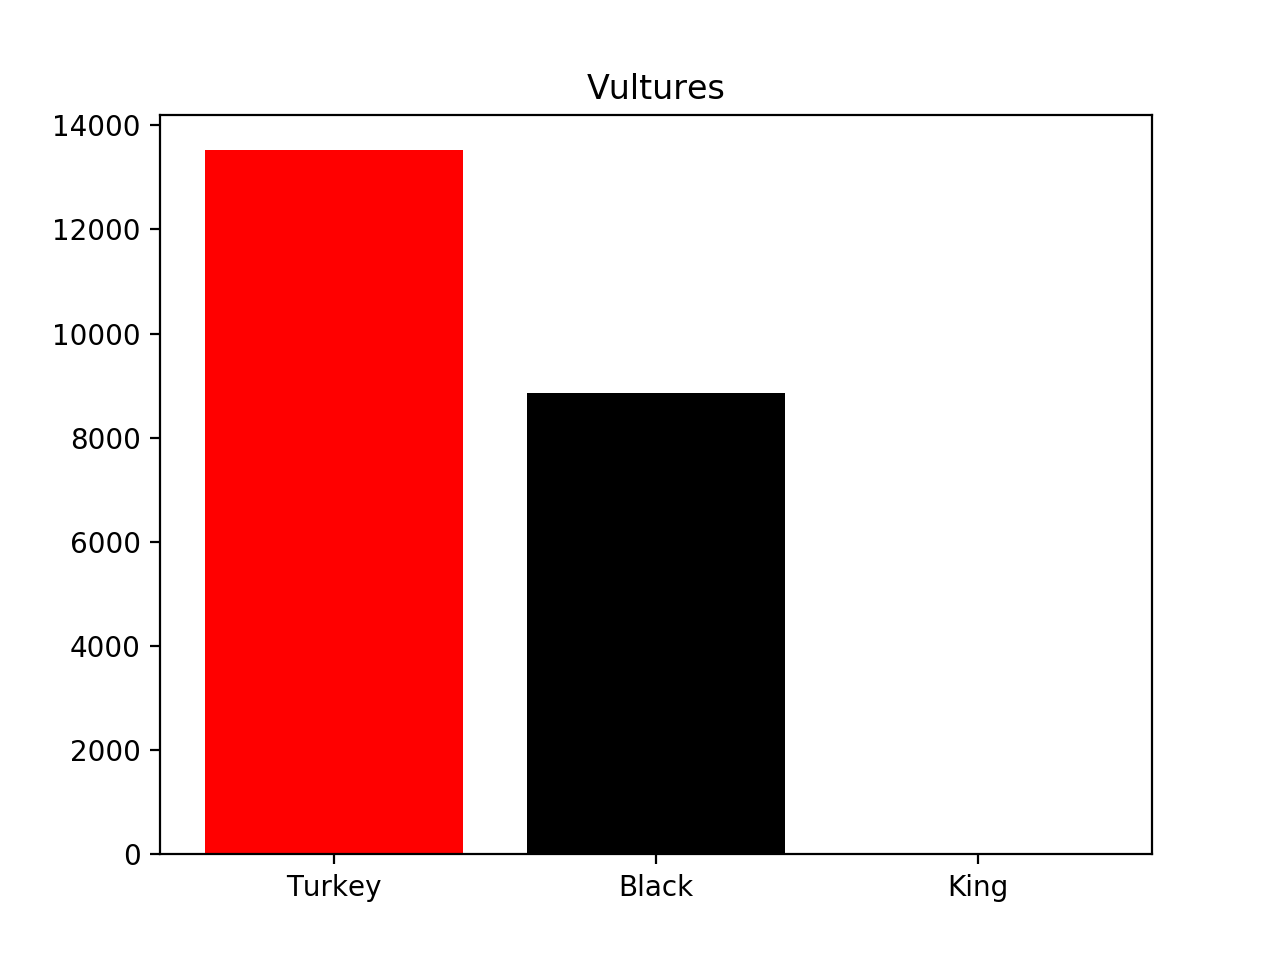
\includegraphics[width=0.5\textwidth]{./figures/prototype-barplot-vultures.png}
%         \caption{Frequencies of Vultures named in Zapotec, with the prototypical Turkey Vulture highlighted in red.}
%         \label{fig-freq-prototype-vultures}
%   \end{center}
% \end{figure}

\begin{figure*}[ht!]
  \begin{center}
    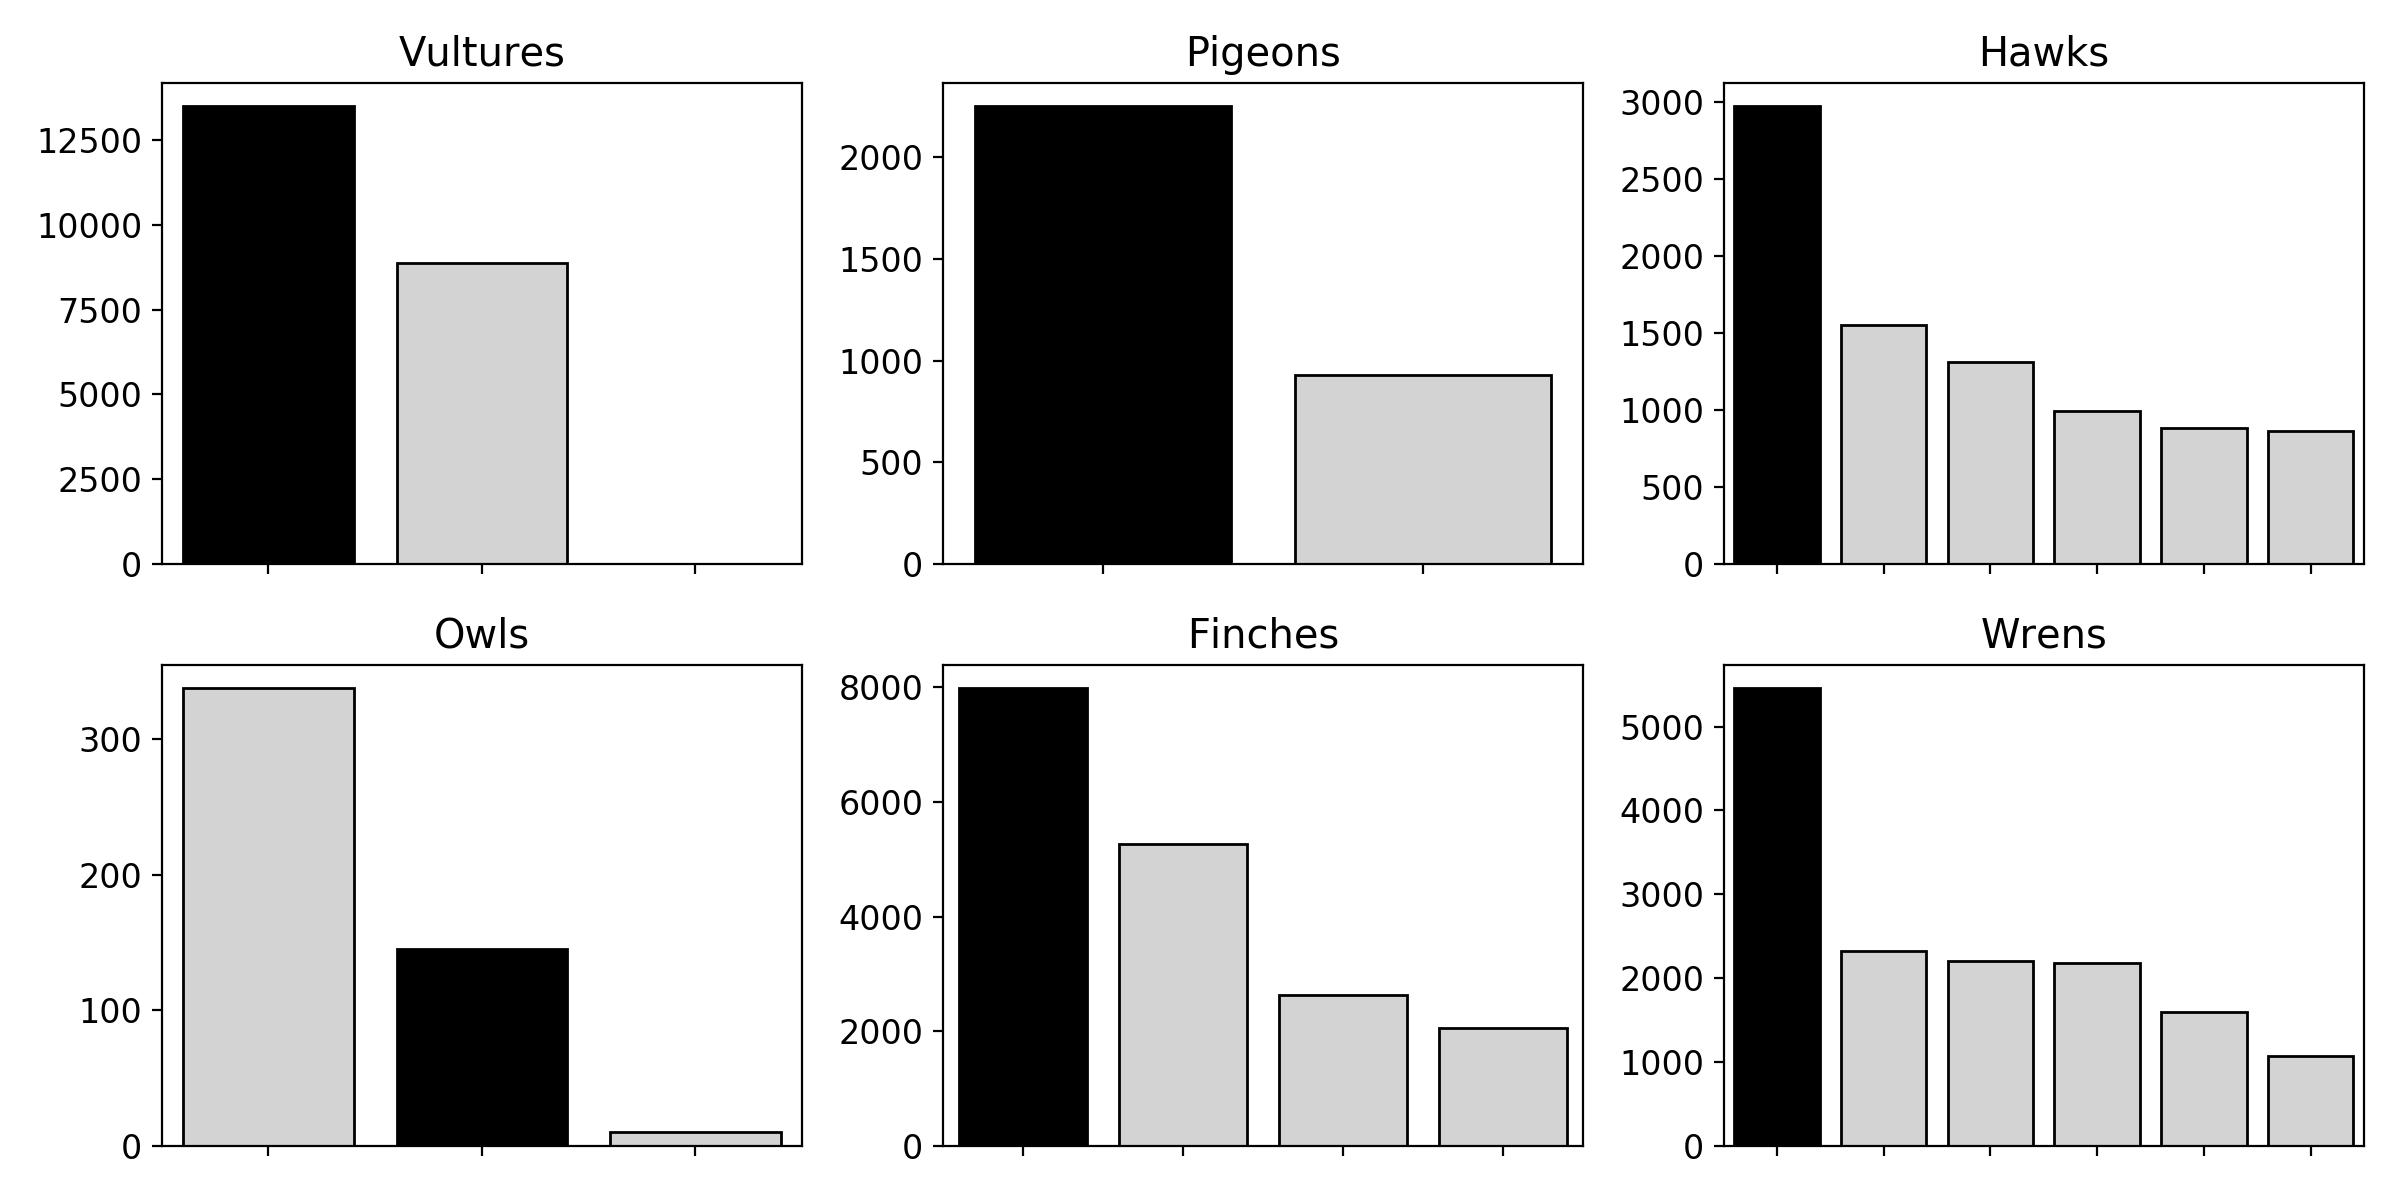
\includegraphics[width=0.95\textwidth]{./figures/prototypes-barplots-all.png}
        \caption{Frequency bar plots of birds named in Zapotec as unmarked prototypes and the frequencies of other birds with the same folk generic name.}
        \label{fig-freq-prototype-all}
  \end{center}
\end{figure*}


We also examined the distribution of the frequencies of birds in Zapotec split into groups based on whether the label is an unmarked prototype or not. We found those that are prototypes are highest in frequency (m=7.93 vs. m=7.02 for log frequency of prototypes and non-prototypes respectively).

% \begin{figure}[ht!]
%   \begin{center}
%     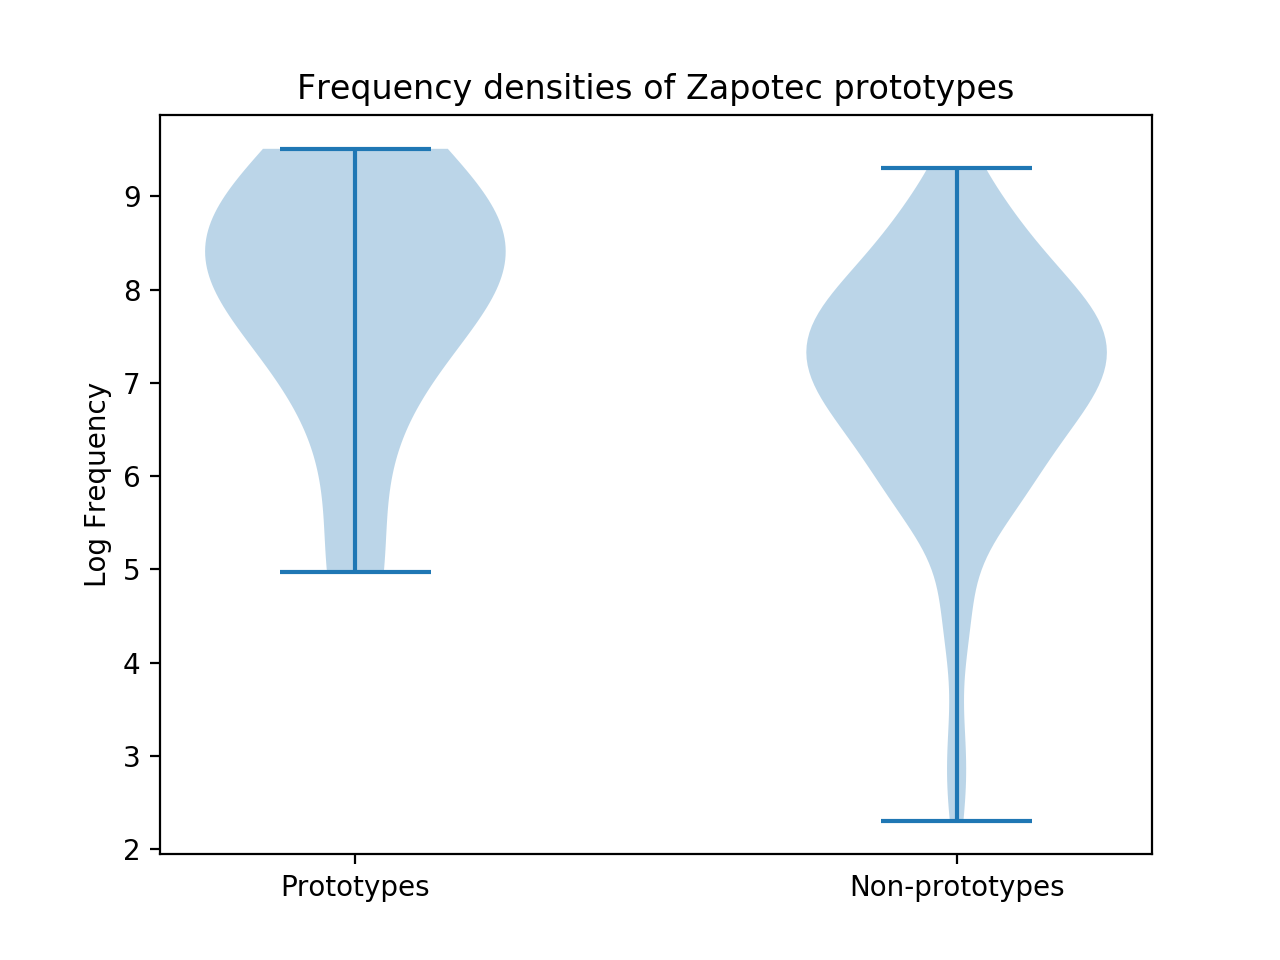
\includegraphics[width=0.5\textwidth]{./figures/prototypefreqs-violinplots.png}
%         \caption{Log-Frequency densities of birds named in Zapotec as a function of whether or not their name is an unmarked-prototype.}
%         \label{fig-freq-prototype-densities}
%   \end{center}
% \end{figure}







\section{Discussion}

% This work extends the investigation of language categories using large-scale datasets online \cite{kemp2012kinship,regier2016languages}
Summary of some of the questions we could explore using the methods detailed above.

\subsection{Potential concerns}

We address potential concerns that can arise in using eBird frequency of observation data here. Does frequency of observation in eBird accurately represent the statistic of interest? (SOME CITATIONS to back up this claim). 

Also, note our observation about the owl prototypes above -- this was an interesting insight which could be backed up by adding additional environmental feature data from EltonTraits \cite{wilman2014eltontraits}, which would indicate that these birds were all nocturnal (and thus potenially more difficult to reflect accurate numbers through eBird).

Also: These questions are interesting because we typically take for granted the categories of natural kinds. However, scientific taxonomies are just another human-constructed category system. When considering the set of birds in particular, it has been difficult for biologists to agree on a standardized taxonomy, which has been shown to severely impact decisions on conservation policy \cite{peterson2006taxonomy,garnett2017taxonomy}.

\subsection{Future Directions}
The next step would be to expand these analyses to more languages. To do this one needs to find trustworthy ethnographies similar to the Zapotec naming data we used here from \citeA{hunn2008zapotec}, and one needs decent coverage in eBird over the geographic region in question. Clear next steps would be to analyze the Tzeltal language from Chiapas, Mexico, and the Tlingit language from the south-east Alaska, both published by Hunn as well \cite{hunn1977tzeltal,hunn2012tlingit}, which have decent coverage within their respective geographics regions in eBird observational data. 

That said, it can be difficult to find languages with both expert ethnographries of the folk biological naming systems which also have good coverage in eBird. This has prohibited us from exploring bird naming data from known experts in regions with low coverage in eBird (e.g., naming data summarized in \cite{holman2002relation}, including the Tobelo language from Indonesia \cite{taylor1990folk} and the Anindilyakwa language from Australia \cite{waddy1988classification}, which do not have coverage in eBird currently).

\section{Conclusion}

% \section{Formalities, Footnotes, and Floats}


% The entire content of a paper (including figures, references, and anything else) can be no longer than six pages in the \textbf{initial submission}. In the \textbf{final submission}, the text of the paper, including an author line, must fit on six pages. Up to one additional page can be used for acknowledgements and references.

% The text of the paper should be formatted in two columns with an
% overall width of 7 inches (17.8 cm) and length of 9.25 inches (23.5
% cm), with 0.25 inches between the columns. Leave two line spaces
% between the last author listed and the text of the paper; the text of
% the paper (starting with the abstract) should begin no less than 2.75 inches below the top of the
% page. The left margin should be 0.75 inches and the top margin should
% be 1 inch.  \textbf{The right and bottom margins will depend on
%   whether you use U.S. letter or A4 paper, so you must be sure to
%   measure the width of the printed text.} Use 10~point Times Roman
% with 12~point vertical spacing, unless otherwise specified.

% The title should be in 14~point bold font, centered. The title should
% be formatted with initial caps (the first letter of content words
% capitalized and the rest lower case). In the initial submission, the
% phrase ``Anonymous CogSci submission'' should appear below the title,
% centered, in 11~point bold font.  In the final submission, each
% author's name should appear on a separate line, 11~point bold, and
% centered, with the author's email address in parentheses. Under each
% author's name list the author's affiliation and postal address in
% ordinary 10~point type.

% Indent the first line of each paragraph by 1/8~inch (except for the
% first paragraph of a new section). Do not add extra vertical space
% between paragraphs.


% \section{First Level Headings}

% First level headings should be in 12~point, initial caps, bold and
% centered. Leave one line space above the heading and 1/4~line space
% below the heading.


% \subsection{Second Level Headings}

% Second level headings should be 11~point, initial caps, bold, and
% flush left. Leave one line space above the heading and 1/4~line
% space below the heading.


% \subsubsection{Third Level Headings}

% Third level headings should be 10~point, initial caps, bold, and flush
% left. Leave one line space above the heading, but no space after the
% heading.


% \section{Formalities, Footnotes, and Floats}

% Use standard APA citation format. Citations within the text should
% include the author's last name and year. If the authors' names are
% included in the sentence, place only the year in parentheses, as in
% \citeA{NewellSimon1972a}, but otherwise place the entire reference in
% parentheses with the authors and year separated by a comma
% \cite{NewellSimon1972a}. List multiple references alphabetically and
% separate them by semicolons
% \cite{ChalnickBillman1988a,NewellSimon1972a}. Use the
% ``et~al.'' construction only after listing all the authors to a
% publication in an earlier reference and for citations with four or
% more authors.


% \subsection{Footnotes}

% Indicate footnotes with a number\footnote{Sample of the first
% footnote.} in the text. Place the footnotes in 9~point font at the
% bottom of the column on which they appear. Precede the footnote block
% with a horizontal rule.\footnote{Sample of the second footnote.}


% \subsection{Tables}

% Number tables consecutively. Place the table number and title (in
% 10~point) above the table with one line space above the caption and
% one line space below it, as in Table~\ref{sample-table}. You may float
% tables to the top or bottom of a column, and you may set wide tables across
% both columns.

% \begin{table}[H]
% \begin{center} 
% \caption{Sample table title.} 
% \label{sample-table} 
% \vskip 0.12in
% \begin{tabular}{ll} 
% \hline
% Error type    &  Example \\
% \hline
% Take smaller        &   63 - 44 = 21 \\
% Always borrow~~~~   &   96 - 42 = 34 \\
% 0 - N = N           &   70 - 47 = 37 \\
% 0 - N = 0           &   70 - 47 = 30 \\
% \hline
% \end{tabular} 
% \end{center} 
% \end{table}


% \subsection{Figures}

% All artwork must be very dark for purposes of reproduction and should
% not be hand drawn. Number figures sequentially, placing the figure
% number and caption, in 10~point, after the figure with one line space
% above the caption and one line space below it, as in
% Figure~\ref{sample-figure}. If necessary, leave extra white space at
% the bottom of the page to avoid splitting the figure and figure
% caption. You may float figures to the top or bottom of a column, and
% you may set wide figures across both columns.

% \begin{figure}[H]
% \begin{center}
% \fbox{CoGNiTiVe ScIeNcE}
% \end{center}
% \caption{This is a figure.} 
% \label{sample-figure}
% \end{figure}


% \section{Acknowledgments}

% In the \textbf{initial submission}, please \textbf{do not include
%   acknowledgements}, to preserve anonymity.  In the \textbf{final submission},
% place acknowledgments (including funding information) in a section \textbf{at
% the end of the paper}.


% \section{References Instructions}

% Follow the APA Publication Manual for citation format, both within the
% text and in the reference list, with the following exceptions: (a) do
% not cite the page numbers of any book, including chapters in edited
% volumes; (b) use the same format for unpublished references as for
% published ones. Alphabetize references by the surnames of the authors,
% with single author entries preceding multiple author entries. Order
% references by the same authors by the year of publication, with the
% earliest first.

% Use a first level section heading, ``{\bf References}'', as shown
% below. Use a hanging indent style, with the first line of the
% reference flush against the left margin and subsequent lines indented
% by 1/8~inch. Below are example references for a conference paper, book
% chapter, journal article, dissertation, book, technical report, and
% edited volume, respectively.

% \nocite{ChalnickBillman1988a}
% \nocite{Feigenbaum1963a}
% \nocite{Hill1983a}
% \nocite{OhlssonLangley1985a}
% % \nocite{Lewis1978a}
% \nocite{Matlock2001}
% \nocite{NewellSimon1972a}
% \nocite{ShragerLangley1990a}

% \newpage
\bibliographystyle{apacite}

\setlength{\bibleftmargin}{.125in}
\setlength{\bibindent}{-\bibleftmargin}

\bibliography{CogSci2020}


\end{document}
